\chapter{实现}
\label{chp:implementation}

\par 在第~\ref{chp:cw-cache}章中我们对问题进行了建模并且对我们提出的Bundle-K的方案做了理论分析,论证了我们的方案的可行性。在本章当中我们会介绍CW-Cache的具体实现。

\section{架构概览}
\label{sec:archi-overview}

\par 我们在~\ref{subsec:alluxio}小节中介绍过的分布式内存文件系统Alluxio上实现了CW-Cache,图~\ref{fig:cw-cache-archi}展示了CW-Cache的整体框架。CW-Cache系统主要由两部分组成:CW-Master和CW-Client,它们分别是在Alluxio Master和Alluxio Client的基础上实现的。

\par CW-Master实现了第\ref{chp:cw-cache}章中描述的Bundle-K方案的主要逻辑,除了原来Alluxio Master具有的响应Client的请求、维护全局的文件的元数据之外,还要记录保存查询任务对数据表中列的访问次数,运行Bundle-K方案中的逻辑对数据表进行列级别的复制,当Client访问数据表中的列的时候返回所有副本所在位置。

\par CW-Client依旧是用户的应用与系统交互的桥梁。CW-Cache接受应用的读/写请求,并与CW-Master交互获得文件所在位置,在执行SQL查询任务的时候,CW-Client会发起远程调用,上传访问的文件的URI、偏移量(Offset)和长度。读取数据表的列所在的文件时,它收到CW-Master传来的副本(原表)所在的位置,根据一定的策略自行决定从哪里读取。此外,图中的应用主要指上层应用框架,比如Spark,Hive等等,通过Alluxio提供的通用接口存取文件。Cache Server上由Alluxio Worker来管理本地节点的文件或者对象。

\begin{figure}[]
	\centering
	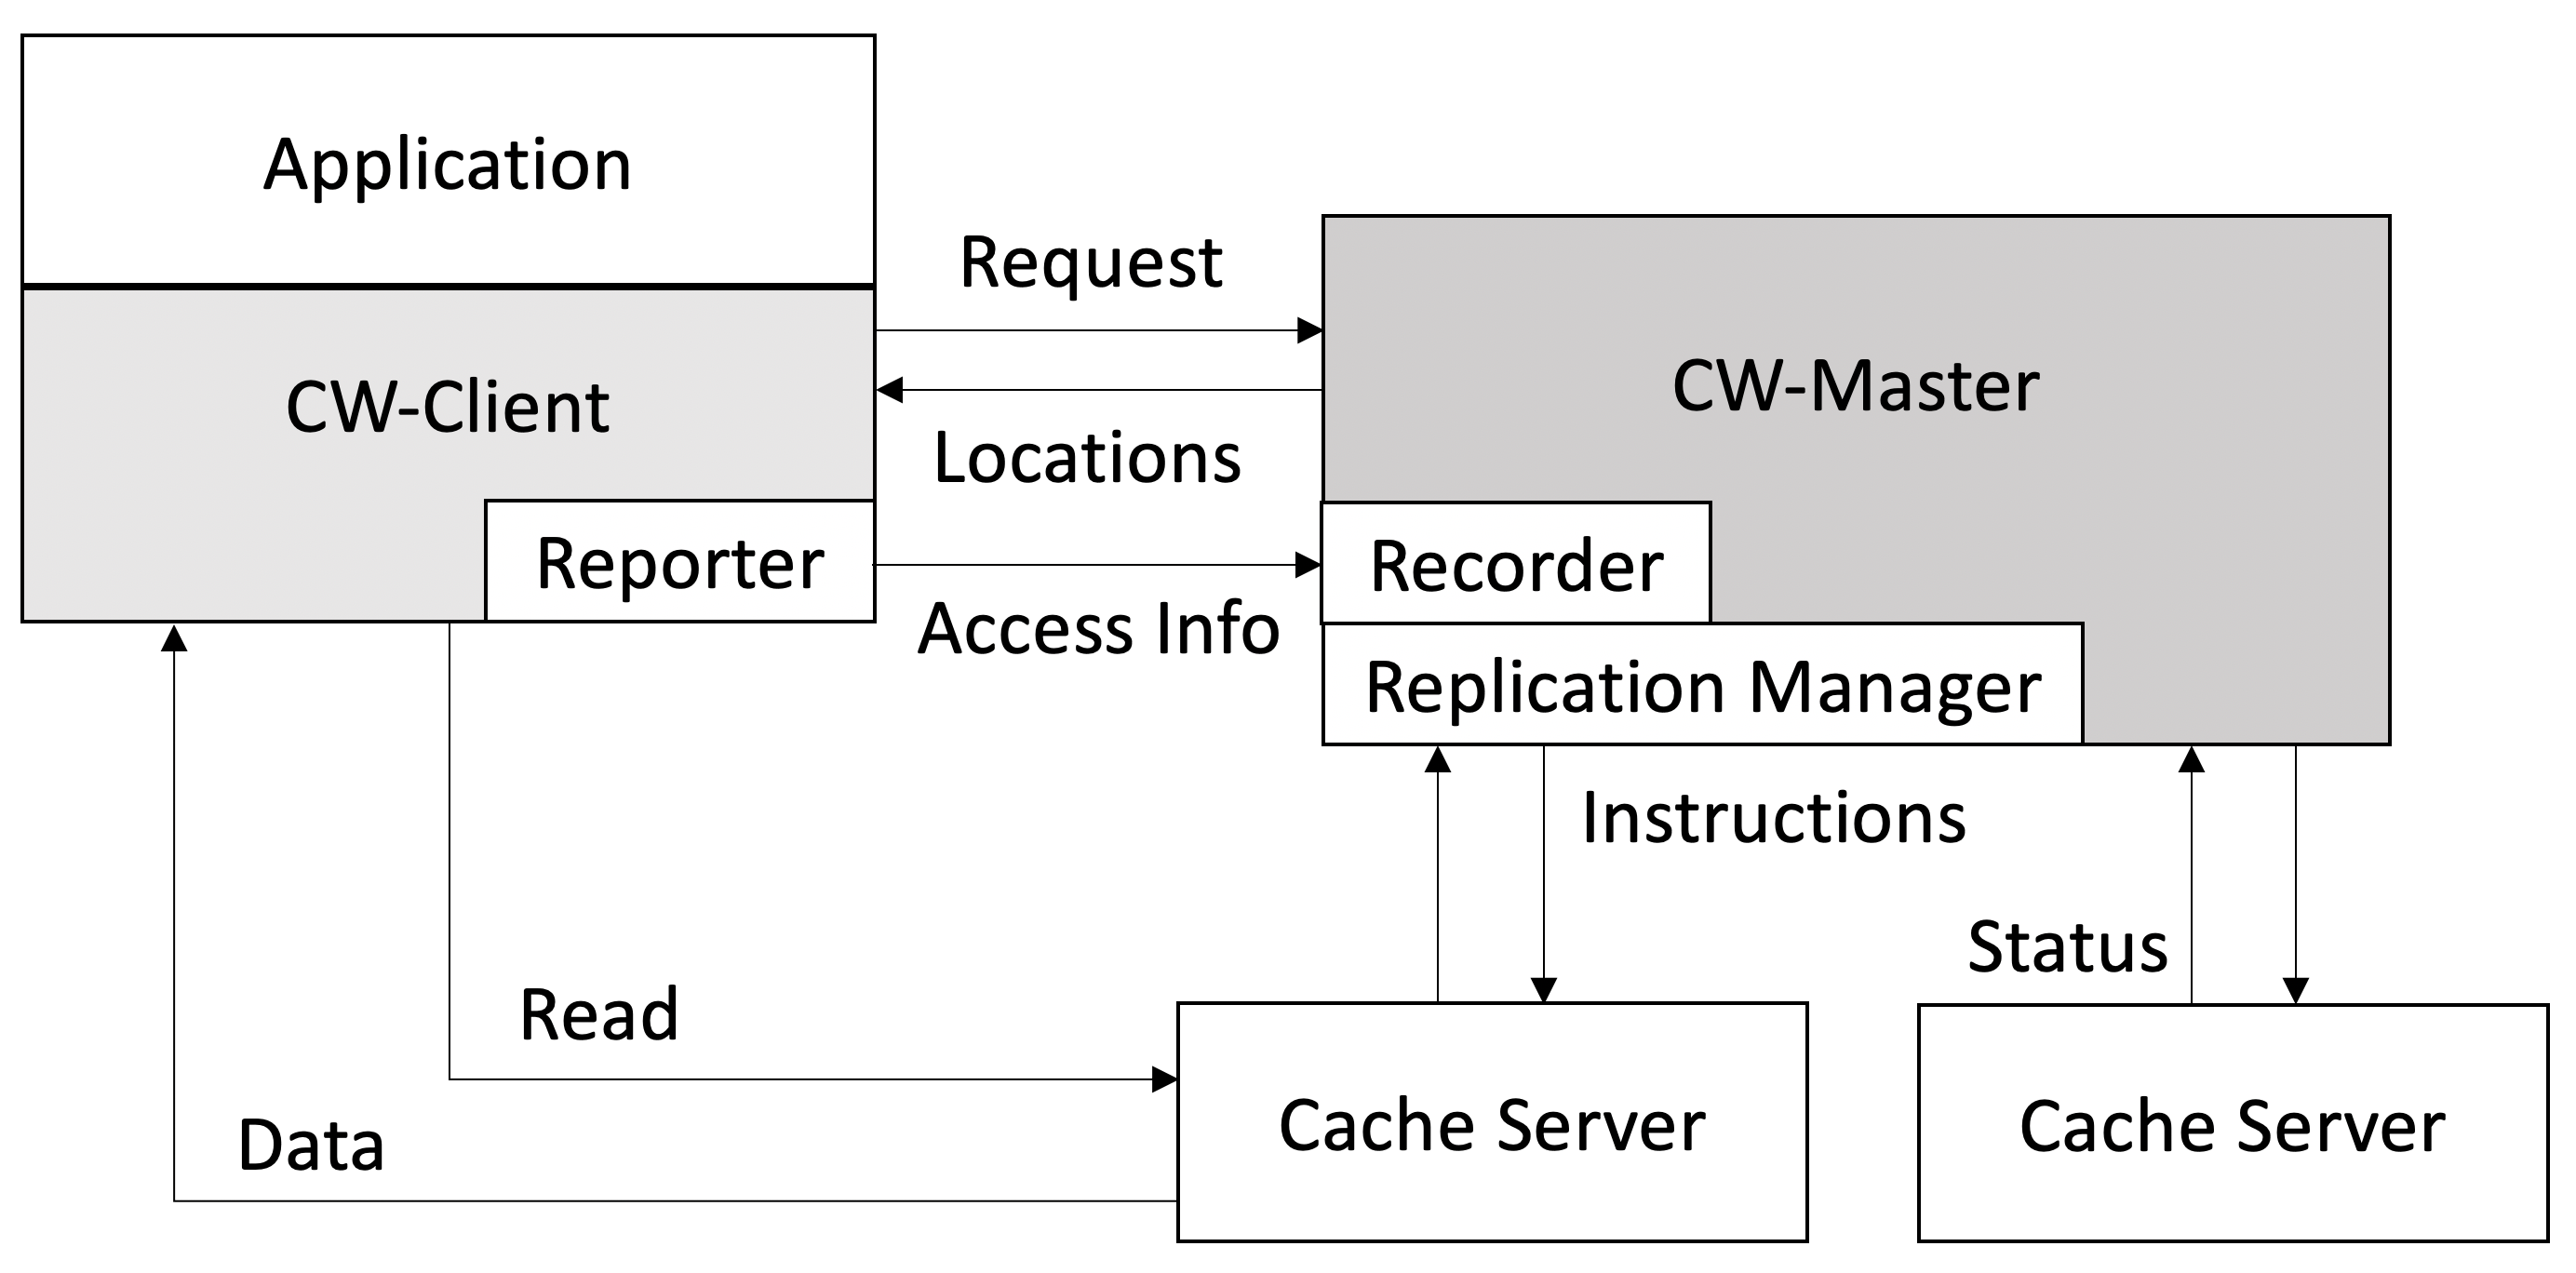
\includegraphics[width=0.8\textwidth]{img/implementation/cw-cache-archi}
	
	\caption{简单方案的架构设计。}
	\label{fig:cw-cache-archi}
	%\vspace{-.1in}
\end{figure}

\par Reporter是增加在Client端用于将应用访问的文件的信息:文件URI,偏移量和长度汇报给Master;Recorder是在Master端用于接收Reporter汇报的数据并将其存储在特定的数据结构中,维护热度的统计信息;Replication Manager负责利用数据表的列的热度数据,执行第~\ref{chp:cw-cache}章中的Bundle-K方案,计算出$K$和复制的份数$r$,对前$K$个最热门列进行“捆绑”复制。此外,Replication Manager也会在CW-Client的读请求到来时返回所有副本(如果有)的位置,供其选择。

\section{实现细节分析}